\documentclass[10pt,a4paper]{article}
\usepackage[utf8]{inputenc}
\usepackage{amsmath}
\usepackage{amsfonts}
\usepackage{amssymb}
\usepackage{graphicx}
\usepackage{float}
\usepackage{url}
\usepackage{graphicx}
\graphicspath{ {images/} }

\title{\textbf{Machine Learning Project} \\ Training Convolutional Neural Networks for Computer Vision using CAD models}
\author{João Belo - 201703263} 

\begin{document}

\maketitle
\begin{abstract}
In 2012 a convolutional neural network (CNN)\cite{krizhevsky2012imagenet} was the winner of the ImageNet image classification challenge, by a considerable margin. Deep Learning has since then revolutionised computer vision. CNN's have been a popular research topic and have been successfully used to solve challenges not only in computer vision but also in other topics such as natural language processing. The goal of this project is to cover the fundamentals of deep learning and explore how to generate synthetic data to train CNN's and solve some image classification challenges that will be discussed in the following section.
\end{abstract}

\section{The Image Classification problem}
Image classification is one of the main problems in computer vision, where the task is to predict a label from a fixed set of categories for an image. Although this is an easy task for an human, for a computer algorithm such a task is not trivial. Taking into account that the representation of images in a computer is a 3-D array of values that go from 0 to 255, one also needs to consider the following challenges\cite{stanfordic}:
\begin{itemize}
\item \textbf{Viewpoint variation} An object can be oriented in different ways with respect to the camera
\item \textbf{Scale variation} A visual class may have different sizes, not only the size in the image but also in the real world.
\item \textbf{Deformation} Some classes don't have rigid bodies, and can be deformed in different ways.
\item \textbf{Occlusion} Objects of interest can be occluded in the picture, and only a small portion of it may be visible
\item \textbf{Illumination conditions} A picture with the same object can be different according to the lighting conditions.
\item \textbf{Background clutter} The objects of interest may blend in the environment.
\item \textbf{Intra-class variation} Objects in the same class may have different appearances
\end{itemize}
A data driven approach has been the most successful at solving Image Classification problems. In this approach, a learning algorithm is trained using a dataset with labelled images and often an algorithm with a lot of data is able to beat a cleverer one with less data\cite{domingos2012few}. The main goal of this project is to perform image classification on objects that can be in different states, and identify these states accordingly (e.g.: when a table is being assembled, identify it and the different steps it goes through whenever a different part is connected). However, gather, clean and integrate the training datasets is a time-consuming task. In this work I will replace the tedious task of putting together this datasets by generating the training data synthetically. Afterwards, this data will be used to train machine learning algorithms to solve the image classification task and analyse how well they perform when making predictions on images from the real world. The problem can be simplified if we split it in the following two image classification problems:

\begin{itemize}
\item Recognizing an object that can be in multiple states among other classes
\item Recognizing the state of an object, where the object is known
\end{itemize}

\section{Convolutional Neural Networks}
In this section I'll go over the fundamentals of Convolutional Neural Networks and briefly cover concepts that are commonly seen in the architecture of popular CNNs and will be used in the implementation of the algorithms for this project.

\subsection{Loss Functions}
Loss functions measure the inconsistency between a given set of parameters and the actual labels in the training dataset - the intuition is that the loss has a high value if the predictions deviate too much from the ground truth and a low value in the opposite case. Hence, they are an important part of neural networks to access the robustness of a model.  Two loss functions commonly used in neural networks are the following:

\subsubsection{Multiclass SVM / Hinge loss}
This loss function expects that the correct class for each prediction is higher than the incorrect classes by a $\Delta$ margin. The mathematical formulation is the following: $$\sum_{j \neq y_i} max (0, s_j - s_{y_i} + \Delta)$$ A variation of this function is the squared hinge, where violated margins are penalized more strongly. 

\subsubsection{Cross Entropy Loss}
This loss function increases as the predicted probability diverges from the actual label. It is particularly useful when we have normalized class probabilities as an output that can be obtained using a Softmax function, since it measures the performance of a classification model whose output is a probability between 0 and 1. The mathematical formulation is the following: $$L_i = -f_{y_i} + log \sum_{j} e^{f_i}$$ Due to numerical instability a normalization trick should be used.

\subsection{Optimization}
Optimization is the process of finding the best parameters in the layers of the CNN to minimize the loss function. A good strategy is to follow the gradient to know in which direction the weights should be updated to minimize the loss function. This takes us the following popular algorithm:

\subsubsection{Mini-batch Gradient Descent + Momentum}
Gradient descent is a procedure where the gradient is evaluated repeatedly and the weights are updated accordingly every step. The size of the step (how much we update the weights) depends on a important hyperparameter - the learning rate. In CNNs, since the datasets are extremely large, it's not computational efficient to compute the gradients on the entire data to update a parameter, therefore the gradient is computed in batches of data. Hence, the name Mini-batch Gradient Descent.

Considering that the function we are trying to optimize is a hilly terrain, there is a chance that we get stuck in a local minima or a saddle point. To achieve better convergence rates, one can add momentum to the existent optimization algorithm. The parameter vector will build up velocity in a direction that has consistent gradient and solve the problem of getting stuck.

There are other good choices of optimization algorithms, such as Adam\cite{kingma2014adam}. However, Mini-batch Gradient Descent + Momentum usually outperform Adam when implemented with weight decay.

\subsection{Backpropragation}
Backpropagation allows us to compute gradients of expressions by applying the chain rule recursively. It consists of two passes: the forward pass, where all the values are computed from the input to the output, and the backward pass, that starts at the end of the model and applies the chain rule to compute the gradients. Platforms such as PyTorch and TensorFlow are capable of performing this step.

\subsection{Architecture}
Convolutional Neural Networks are made up of a sequence of different types of layers. The main types of layers used in CNN architectures are the following:

\subsubsection{Fully connected layers}
These are the layers that are seen in regular neural networks, where the neurons are in a fully connected layer with full connections to all the activations in the previous layer. Typically, there is at some point a transition to fully connected layers where the last layer holds the output of the network.

\subsubsection{Convolution layers}
The parameters of convolutional layers consist of learnable filters. Each of these filters corresponds to a small spatial position on the input and by sliding the filter through the image a 2-dimensional activation map is produced. This will allow the network to activate the filters according to some learned visual features (e.g.: edges or patterns). The layers have three important hyperparameters, that control the size of the output volume:
\begin{itemize}
\item \textbf{Depth} - can be interpreted as the number of features we would like to learn from a specific spacial position from the image. 
\item \textbf{Stride} - This parameter refers to how much the filter is moved between each image.
\item \textbf{Zero padding} - Sometimes it is necessary to add padding around the border of the input image to control the size of the output volumes.
\end{itemize}

\subsubsection{Pooling layers}
Pooling layers are common in-between convolution layers. They reduce the spacial size of the representation and reduce the amount of parameters and computation in the network. In these layers a spatial region is reduced in dimensions by typically taking the maximum value (max pooling). There are other possible functions such as average pooling, but max pooling has proven to be the most successful.

\subsection{Regularization}
Regularization can be very useful to prevent the model from overfitting. This can be done by simply extending the loss function with a regularization penalty R(W). The most common one is the L2 norm that discourages large weights in the model: $$ R(W) = \sum_{k} \sum_{l} W_{k,l}^2$$ However, other recent techniques can contribute to achieving better results:

\subsubsection{Dropout}
When using dropout, some neurons will only remain active with a probability \textit{p}. This reduces node interactions, leading them to learn more robust features.

\subsubsection{Batch Normalization}
Batch normalization\cite{ioffe2015batch} is a technique that not only acts as a regularizer, but also allows for better initialization. As the name indicates, normalization is performed for each mini-batch, normalizing the input layer by adjusting and scaling the activations. By forcing the activations through the network to take on a unit gaussian distribution the problem caused by the distribution of inputs during training is solved and higher learning rates are possible. 

\subsection{Activation functions}
The output of a node in a neural network is defined by its activation function. This output is then used as the input in the following layer of the network. There are various different activation functions, but I will only cover the  ones that are often used in convolutional neural networks:

\subsubsection{ReLU}
The ReLU activation function is defined as follows: $$f(x) = max(0, x)$$ It's extremely used since it does not saturate in the positive region when compared to other functions such as the sigmoid, it's computationally efficient and converges faster than the sigmoid and tahn activation functions in practice. However, when x is smaller than zero there is a problem with this activation function - the slope will also be zero and the node will not activate or update again. This is also called the "dead ReLU" problem.

\subsubsection{Leaky ReLU}
The leaky ReLU activation function offers a solution to the dead ReLU problem: $$f(x) = max (\alpha x, x)$$
Since the slope is no longer zero, the node can still be updated solving the problem discussed above.

\subsection{Initialization}
To train a network it's necessary to initialize its parameters before. Bad initializations can lead to different issues such as vanishing or exploding gradients. One can avoid these problems by using some of the concepts described in previous sections. A good approach is to use ReLU / Leaky ReLU as the activation function (due to how they affect the gradients). Batch Normalization also makes the CNNs more robust to bad initializations.

\subsubsection{Transfer Learning}
Since it's rare to have a dataset that is large enough to train a CNN, it is common to use a CNN trained on a large dataset (e.g.: ImageNet) and use it as an initialization or a fixed feature extractor.\cite{stanfordtf} These are the common approaches to the 4 major scenarios:
\begin{itemize}
\item \textit{Dataset is small and similar to original dataset} - Train a linear classifier on the CNN nodes.
\item \textit{Dataset is large and similar to original dataset} - Fine-tune through the full network.
\item \textit{Dataset is small but different than the original dataset} - Train the classifier from activations earlier in the network.
\item \textit{Dataset is large but different than the original dataset} - Initialize weights from a pretrained model.
\end{itemize} 
	
\section{Data Generation}
One of the main goals of this project is to generate synthetic training data. This is motivated by the need of large datasets to train CNNs for image classification tasks and is particularly useful when data for a more specific image class is not available. In this project I'll explore efficient ways of generating data of objects that are common in industry or easy to 3D print. This is relevant to my field of studies - object recognition enables new possibilities in augmented reality systems such as context awareness and tracking.

\subsection{Object representation}
CAD models are widely used in industry to represent objects. We can divide this CAD model files in two types: native - particular to a certain CAD software - and neutral - designed for interoperability among software. Hence, since the objective is to render images that are photorealistic it's necessary to find a representation that is both supported by most CAD software where this models are generated, but also on software that can be imported by rendering software. A format that suits this needs is \textit{.obj}. It represents the 3D geometry of the object and in contrast to other popular formats (such as \textit{.slt} for 3D printing) it also supports color and texture information which can be used for rendering\cite{objspec}.

In this project I decided to render a piece of Ikea furniture (Lack Side Table)\cite{lacktable} for the following three reasons:
\begin{itemize}
\item It needs to be assembled, so it has different stages
\item It's a common piece of furniture so it is easy to find its CAD model online
\item It's affordable and easy to buy,  making it possible to take pictures in the real world to test how well our model performs.
\end{itemize}

\subsection{Rendering}
We want to render a dataset that is large enough to train our CNN, therefore it's necessary to find a rendering engine that supports scripting or this task would be just as tedious as gathering data ourselves. Blender is a free and open-source 3D graphics engine that supports python scripting, and fits all the rendering needs for this task. This are picture of the furniture I will render from the Ikea catalogue:

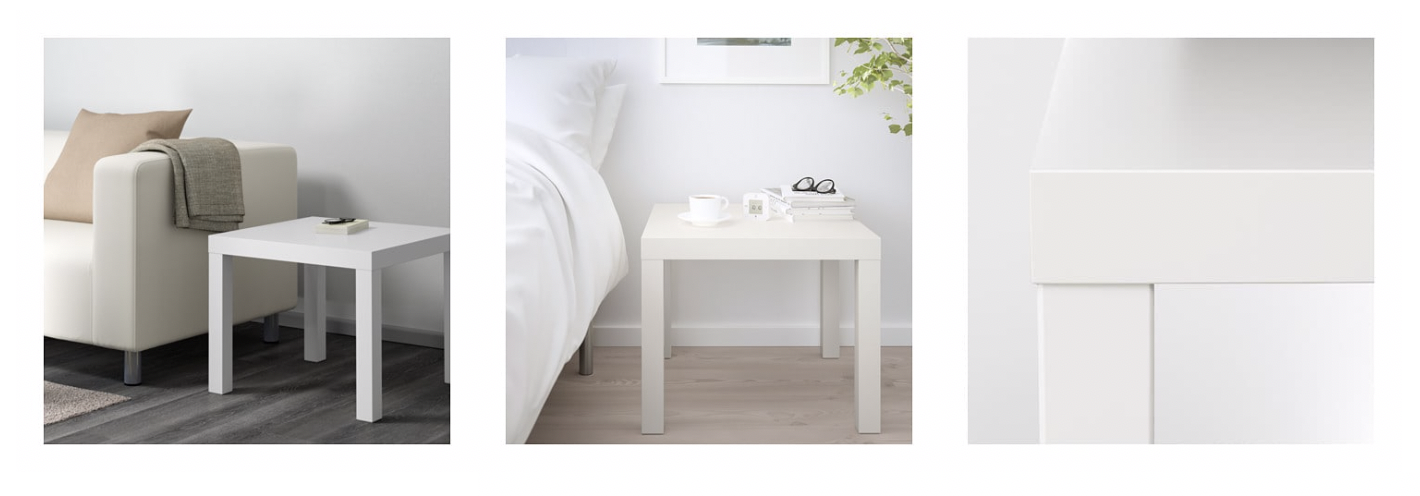
\includegraphics[scale=0.45]{table_3}

In this process it's necessary to take the image recognition challenges into consideration:
\begin{itemize}
\item \textbf{Viewpoint variation} Since the object can be oriented in different in relation to the camera we also have to render it from different camera orientations.
\item \textbf{Scale variation} The size of the object we want to recognize doesn't change in the real world, but it's distance to the camera still has to be taken into consideration.
\item \textbf{Deformation} This is not an issue with this piece of furniture.
\item \textbf{Occlusion} Although occlusion can be a problem, this is something than can be solved by occluding parts of the rendered image later on. The initial objective is to recognize the table without occlusion.
\item \textbf{Illumination conditions} Lighting is an important part of the rendering process and different illumination conditions will be taken into account.
\item \textbf{Background clutter} To deal with this problem background can be added when rendering the object.
\item \textbf{Intra-class variation} If we consider the different stages during assembly, all these stages have to be rendered to identify the object among other classes.
\end{itemize}
For this project, all the images were rendered from the terminal, using a python script. This means that a scene is set up from scratch in Blender and the object we want to render is imported and adjusted accordingly. Afterwards, three lamps are added using the three point lighting method to illuminate the object and one is added on a random position. Several possible starting positions for the camera are defined and for each of them, the object is rendered in 360 degrees. This solves the viewpoint variation and scale variation challenges. The light intensity and position is also changed at random every time the object is rendered, solving the illumination issue. Finally, the object is also rendered in all the different possible stages, by removing the corresponding parts in the CAD model and solve the intra-class variation issues to distinguish our table in different states from other image classes. This are some examples of images we obtain by running the data\_generation.py script in the appendix:

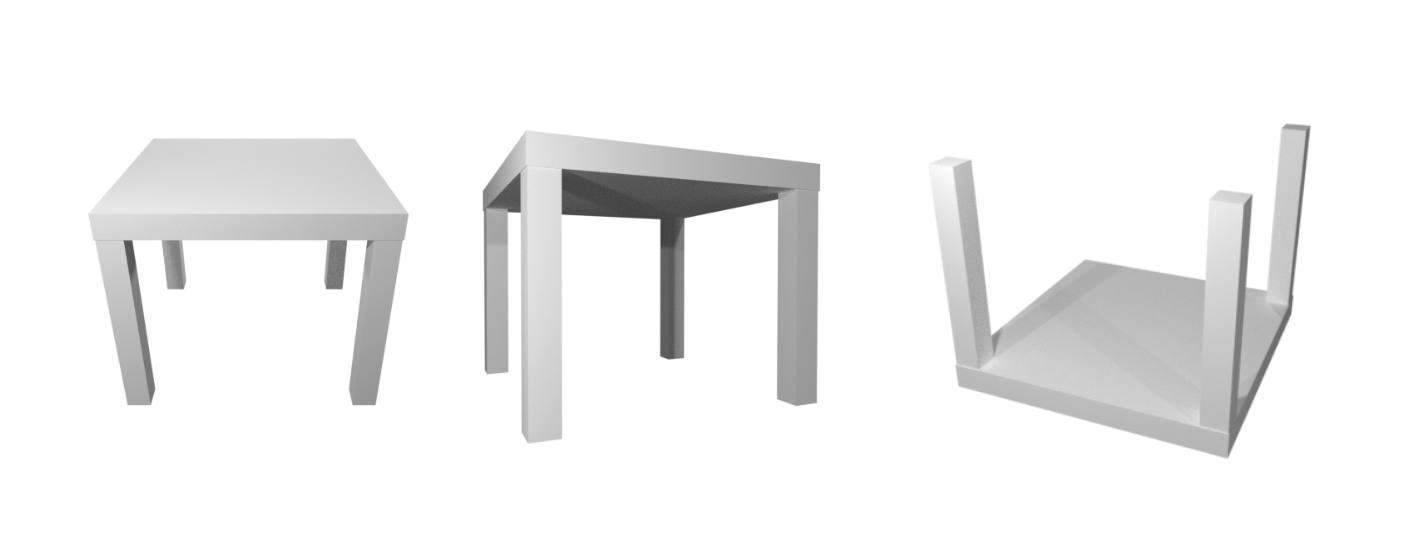
\includegraphics[scale=0.45]{table_1}

The background could also have been added during rendering, but adding more content to the rendered scene would increase the rendering time, and although it would give a more photorealistic result, it would also increase the workload. Therefore I decided to output the generated images in a format with transparency and simply add a random texture in the background. The script to perform this operation uses the python PIL library and is included in the appendix (data\_augmentation.py). These are some examples of the images that are going to be used during training:

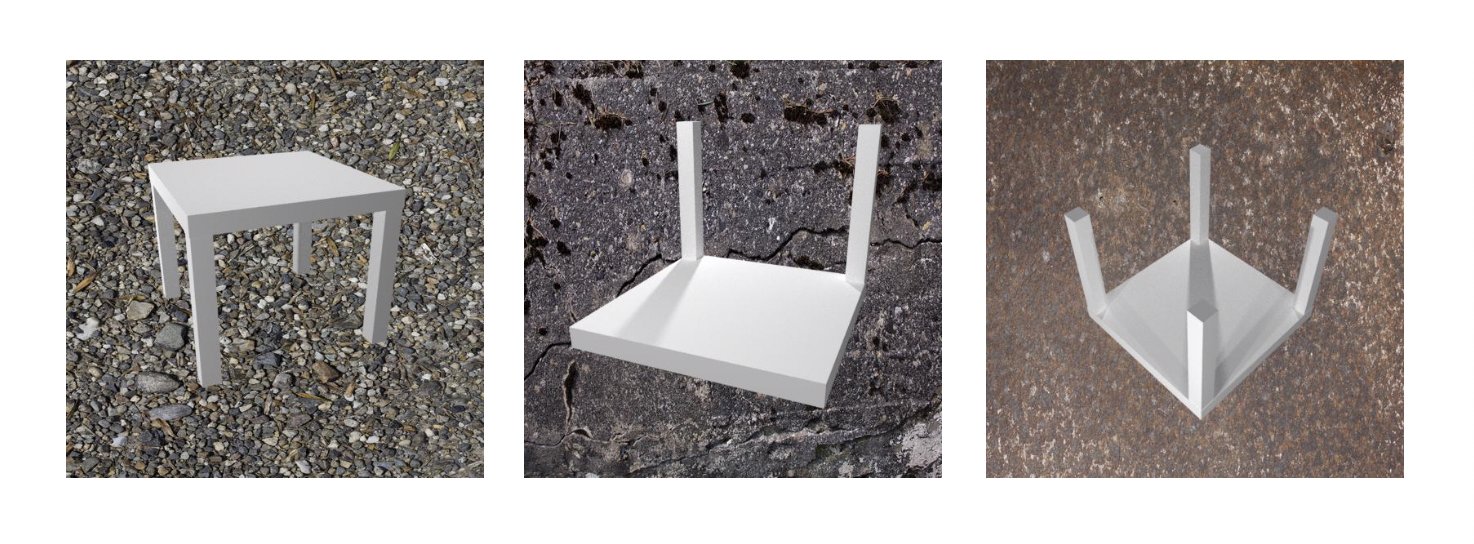
\includegraphics[scale=0.45]{table_2}

The photorealism of the generated images is something that can be improved in future work. Possible improvements would be:
\begin{itemize}
\item Render the object in a complete scene to have more realistic lighting, shadows and background.
\item Better textures/materials for the object.
\item Render each image for a longer period of time.
\end{itemize}

\section{Experiments}
In the experiments I'll see how well convolutional neural networks trained on the generated data perform when classifying real world images of the Ikea table. From now on I will call it by its model name - Lack Table. Hence, I will train two models that perform the following classification tasks:

\begin{itemize}
\item Classify real world pictures of different types furniture, being the Lack Table one of these classes.
\item Classify real world pictures of different stages of assembly of the Lack Table. 
\end{itemize}

To implement the CNN's I will be using PyTorch, a popular open source deep learning platform.

\subsection{Task 1 - Furniture Classifier}


\bibliographystyle{abbrv}
\bibliography{references}
\end{document}
